\begin{center}
\subsection*{Corrig{\'e} de l'{\'e}preuve math{\'e}matiques \ A - \\ XLSR - Fili{\`e}re MP-MPI\\ 2023}\label{mathA_2023}
\textbf{SABIR ilyass - ETTOUSY BADR}
\end{center}
\[
\star \star \star
\]
\addcontentsline{toc}{subsection}{Corrig{\'e} de l'{\'e}preuve math{\'e}matiques \ A - XLSR - Fili{\`e}re MP-MPI 2023}

\subsubsection*{1. Pr{\'e}liminaires}

\

\tmtextbf{1.a. }Montrons que $\mathbb{H}$ est un sous-$\mathbb{R}$
alg{\`e}bre de $M_2 (\mathbb{C})$ stable par $Z \longmapsto Z^{\ast}$.

On a $E = Z (1, 0) \in \mathbb{H}$, et pour tout $z_1, z_2, z_3, z_4 \in
\mathbb{C}$ et $\lambda \in \mathbb{R}$, on a :
\begin{eqnarray*}
  Z (z_1, z_2) + \lambda Z (z_3, z_4) & = & \left(\begin{array}{cc}
    z_1 + \lambda z_3 & - (\overline{z_2 + \lambda z_4})\\
    z_2 + \lambda z_4 & \overline{z_1 + \lambda z_3}
  \end{array}\right)\\
  & = & Z (z_1 + \lambda z_3, z_2 + \lambda z_4)\\
  & \in & \mathbb{H}
\end{eqnarray*}


De plus,
\[ Z (z_1, z_2) \times Z (z_3, z_4) = \left(\begin{array}{cc}
     z_1 z_3 - \bar{z}_2 z_4 & - (\overline{z_2 z_3 + \bar{z}_1 z_4})\\
     z_2 z_3 + \bar{z}_1 z_4 & \overline{z_1 z_3 - \bar{z}_2 z_4}
   \end{array}\right) \in \mathbb{H}. \]


Donc, $\mathbb{H}$est un sous $\mathbb{R}$-alg{\`e}bre de $M_2 (\mathbb{C})$.

Ensuite, on a
\begin{eqnarray*}
  Z (z_1, z_2)^{\ast} & = & \left(\begin{array}{cc}
    \overline{z_1} & \bar{z}_2\\
    - z_2 & z_1
  \end{array}\right)\\
  & = & Z (\overline{z_1}, - z_2)\\
  & \in & \mathbb{H}
\end{eqnarray*}


D'o{\`u} $\mathbb{H}$ est stable par \ $Z \longmapsto Z^{\ast}$.

\

\tmtextbf{1.b.} Soit $Z \in \mathbb{H}$, notons $Z = Z (z_1, z_2)$ o{\`u}
$z_1, z_2 \in \mathbb{C}$.

On a
\begin{eqnarray*}
  Z (z_1, z_2) Z (z_1, z_2)^{\ast} & = & \left(\begin{array}{cc}
    z_1 & - \bar{z}_2\\
    z_2 & \overline{z_1}
  \end{array}\right) \left(\begin{array}{cc}
    \overline{z_1} & \bar{z}_2\\
    - z_2 & z_1
  \end{array}\right)\\
  & = & \left(\begin{array}{cc}
    | z_1 |^2 + | z_2 |^2 & 0\\
    0 & | z_1 |^2 + | z_2 |^2
  \end{array}\right)\\
  & = & (| z_1 |^2 + | z_2 |^2) E
\end{eqnarray*}


De plus, on a
\begin{eqnarray*}
  Z^{\ast} Z & = & Z (\overline{z_1}, - z_2) Z (\overline{z_1}, -
  z_2)^{\ast}\\
  & = & (| \overline{z_1} |^2 + | - z_2 |^2) E\\
  & = & (| z_1 |^2 + | z_2 |^2) E
\end{eqnarray*}


Si $Z (z_1, z_2)$ est non nul, alors $(z_1, z_2) \neq (0, 0)$, en particulier
$| z_1 |^2 + | z_2 |^2 > 0$, d'o{\`u} $Z$ est inversible.

\

\tmtextbf{1.c.} Soit $Z (z_1, z_2) \in \mathbb{H}$, avec $z_1, z_2 \in
\mathbb{C}$.

Si $Z \in \mathbb{R}_{\mathbb{H}},$ alors il existe $a \in \mathbb{R}$ tel que
$Z = a E$.

On a, pour tout $Z' \in \mathbb{H}$,
\begin{eqnarray*}
  Z.Z' & = & a Z'\\
  & = & Z' .Z
\end{eqnarray*}


R{\'e}ciproquement, si pour tout $Z' \in \mathbb{H}$, on a $Z.Z' = Z' .Z$,

Donc, pour tout $z_3, z_4 \in \mathbb{C}$, on a
\[ Z (z_1 z_3 - \bar{z}_2 z_4, z_2 z_3 + \bar{z}_1 z_4) = Z (z_3 z_1 -
   \bar{z}_4 z_2, z_4 z_1 + \bar{z}_3 z_2) \]


Ainsi,
\[ \left\{\begin{array}{l}
     z_1 z_3 - \bar{z}_2 z_4 = z_3 z_1 - \bar{z}_4 z_2\\
     z_2 z_3 + \bar{z}_1 z_4 = z_4 z_1 + \bar{z}_3 z_2
   \end{array}\right. \]


Par suite, pour tout $z_4 \in \mathbb{R}$, on a
\[ z_4 (\bar{z}_2 - z_2) = 0 \]


et pour tout $z_4 \in i\mathbb{R}$, on a
\[ z_4 (\bar{z}_2 + z_2) = 0 \]


En particulier, $z_2 \in \mathbb{R} \cap i\mathbb{R}= \{ 0 \}$, donc $z_2 =
0$.

Et $z_4 (z_1 - \bar{z}_1) = 0$, et {\c c}a pour tout $z_4 \in \mathbb{C},$
donc $z_1 \in \mathbb{R}.$

D'o{\`u}
\[ Z = z_1 .E \in \mathbb{R}_{\mathbb{H}} \]


D'o{\`u} l'{\'e}quivalence.

\

\tmtextbf{2.a.} Pour tout $Z = (z_1, z_2) \in \mathbb{H}$ et $Z' = (z_3, z_4)
\in \mathbb{H}$. On a :
\begin{eqnarray*}
  N (Z Z') & = & N (Z (z_1 z_3 - \bar{z}_2 z_4, z_2 z_3 + \bar{z}_1 z_4))\\
  & = & | z_1 z_3 - \bar{z}_2 z_4 |^2 + | z_2 z_3 + \bar{z}_1 z_4 |^2\\
  & = & | z_1 z_3 |^2 - 2 z_1 z_3 \overline{\bar{z}_2 z_4} + | \bar{z}_2 z_4
  |^2 + | z_2 z_3 |^2 + 2 z_2 z_3 \overline{\bar{z}_1 z_4} + | \bar{z}_1 z_4
  |^2\\
  & = & | z_1 |^2 | z_3 |^2 + | z_2 |^2 | z_4 |^2 + | z_2 |^2 | z_3 |^2 + |
  z_1 |^2 | z_4 |^2\\
  & = & (| z_1 |^2 + | z_2 |^2) (| z_3 |^2 + | z_4 |^2)\\
  & = & N (Z) N (Z')
\end{eqnarray*}


\tmtextbf{2.b.} Montrons que $S$ est un sous groupe de $\mathbb{H}^{\times}$.

On a $N (E) = 1$, donc $E \in S$.

Soient $Z, Z' \in S$. On a $Z, Z' \in \mathbb{H}$ tels que
\begin{eqnarray*}
  N (Z) & = & N (Z')\\
  & = & 1
\end{eqnarray*}


D'apr{\`e}s la question 1.b, on a $Z$ et $Z'$ sont inversibles.

Or, d'apr{\`e}s la question pr{\'e}c{\'e}dente, on a :
\begin{eqnarray*}
  N \left( {Z'}^{- 1} \right) & = & N (Z') .N \left( {Z'}^{- 1} \right)\\
  & = & N \left( Z' {Z'}^{- 1} \right)\\
  & = & N (E)\\
  & = & 1
\end{eqnarray*}


Donc,
\begin{eqnarray*}
  N \left( {Z.Z'}^{- 1} \right) & = & N (Z) N \left( {Z'}^{- 1} \right)\\
  & = & 1
\end{eqnarray*}


Ainsi, ${Z.Z'}^{- 1} \in S$. Donc $S$ est un sous-groupe de
$\mathbb{H}^{\times}$.

De plus, pour tout $Z = (z_1, z_2) \in \mathbb{H}^{\times}$, on a $N (Z) > 0$,
et
\begin{eqnarray*}
  N \left( \frac{1}{\sqrt{N (Z)}} Z \right) & = & \left| \frac{z_1}{\sqrt{N
  (Z)}} \right|^2 + \left| \frac{z_2}{\sqrt{N (Z)}} \right|^2\\
  & = & \frac{1}{N (Z)} N (Z)\\
  & = & 1
\end{eqnarray*}


Donc $\frac{1}{\sqrt{N (Z)}} Z \in S$.

\

\tmtextbf{3.a.} Soient $x, y, z, t \in \mathbb{R}$, on a :
\begin{eqnarray*}
  N (x E + y I + z J + t K) & = & N \left( \left(\begin{array}{cc}
    x + i y & z - i t\\
    - z + i t & x - i y
  \end{array}\right) \right)\\
  & = & | x + i y |^2 + | - z + i t |^2\\
  & = & x^2 + y^2 + z^2 + t^2
\end{eqnarray*}


\tmtextbf{3.b.} Soit $U \in \mathbb{H}^{\tmop{im}}$, on a alors l'existence de
$x, y, z \in \mathbb{R}$ tels que $U = x I + y J + z K$. On a alors :
\begin{eqnarray*}
  U^2 & = & - (x^2 + y^2 + z^2) E\\
  & = & - N (U) E
\end{eqnarray*}


On a donc
\[ \mathbb{H}^{\tmop{im}} \subset \{ \nobracket U \in \mathbb{H} | U^2 \in] -
   \infty, 0] E \} \]


Soit $U \in \mathbb{H}$ tel que $\nobracket \nobracket U^2 \in] - \infty, 0]
E$. Montrons que $U \in \mathbb{H}^{\tmop{im}}$.

On a l'existence de $x, y, z, t \in \mathbb{R}$ tels que
\[ U = x E + y I + z J + t K \]


On a :
\[ U^2 = (x^2 - y^2 - z^2 - t^2) E + 2 x y I + 2 x z J + 2 x t K \]


On a $\nobracket \nobracket U^2 \in] - \infty, 0] E$, donc $x y = x z = x t =
0$ et $x^2 \leqslant y^2 + z^2 + t^2$.

Si $x \neq 0$, alors $y = z = t = 0$. Par suite $x^2 \leqslant 0$, donc $x =
0$, ce qui est absurde.

D'o{\`u} $x = 0$. Par suite
\[ U = y I + z J + t K \in \mathbb{H}^{\tmop{im}} \]


\tmtextbf{4.} On a $Z \in \mathbb{H} \rightarrow \sqrt{N (Z)}$ est une norme
sur $\mathbb{H}$ associ{\'e}e au produit scalaire $\langle ., . \rangle$.

On a $S$ est la sph{\'e}re unit{\'e} centr{\'e}e en $0$ de l'espace vectoriel
norm{\'e} $\left( \mathbb{H}, \sqrt{N} \right)$.

Ainsi, $S$ est un ferm{\'e} de $\mathbb{H}$, et on a
\[ \psi (\{ (x, y, z, t) \in \mathbb{R}^4 | x^2 + y^2 + z^2 + t^2 = 1
   \nobracket \}) = S \]


Or, $\{ (x, y, z, t) \in \mathbb{R}^4 | x^2 + y^2 + z^2 + t^2 = 1 \nobracket
\}$ est la sph{\'e}re unit{\'e} centr{\'e}e en 0 de $\mathbb{R}^4$, qui est
donc connexe par arcs.

De plus, $\psi$ est 1-lipschitzienne, donc en particulier qu'elle est
continue.

Ainsi, $S$ est connexe par arc, comme {\'e}tant l'image directe par une
application continue d'une partie connexe par arcs.

\

\tmtextbf{5.} Soient $U, V \in H^{\tmop{im}}$.

\tmtextbf{5.a.} Montrons que $U$ et V sont orthogonaux si et seulement si $U V
+ V U = 0$.

Supposons que $U$ et V sont orthogonaux. On a
\begin{eqnarray*}
  U V + V U & = & (U + V)^2 - U^2 - V^2\\
  & = & - (N (U + V) - N (U) - N (V)) E
\end{eqnarray*}


Donc, $U$ et V sont orthogonaux si et seulement si
\[ N (U + V) = N (U) + N (V) \]


ce qui est {\'e}quivalent {\`a} $U V + V U = 0$.

Dans ce cas, on a
\begin{eqnarray*}
  (U V)^2 & = & - U V^2 U\\
  & = & N (V) U^2\\
  & = & - N (U) N (V) E
\end{eqnarray*}


avec
\[ - N (U) N (V) \leqslant 0 \]


Donc $U V \in H^{\tmop{im}}$.

Notons
\[ U = x_1 I + y_1 J + z_1 K \]


et
\[ V = x_2 I + y_2 J + z_2 K \]


avec $x_1, x_2, y_1, y_2, z_1, z_2 \in \mathbb{R}$.

On obtient alors
\begin{eqnarray*}
  U V & = & (y_1 z_2 - z_1 y_2) I + (z_1 x_2 - x_1 z_2) J + (x_1 y_2 - y_1
  x_2) K
\end{eqnarray*}


(car $U$ et V sont orthogonaux).

Ainsi, la matrice de $(U, V, U V)$ dans la base $(I, J, K)$ est
\[ \left(\begin{array}{ccc}
     x_1 & x_2 & y_1 z_2 - z_1 y_2\\
     y_1 & y_2 & z_1 x_2 - x_1 z_2\\
     z_1 & z_2 & x_1 y_2 - y_1 x_2
   \end{array}\right) \]


Avec
\[ \left(\begin{array}{c}
     x_1\\
     y_1\\
     z_1
   \end{array}\right) \wedge \left(\begin{array}{c}
     x_2\\
     y_2\\
     z_2
   \end{array}\right) = \left(\begin{array}{c}
     y_1 z_2 - z_1 y_2\\
     y_1 z_2 - z_1 y_2\\
     x_1 y_2 - y_1 x_2
   \end{array}\right) \]


Donc, le d{\'e}terminant de $\left(\begin{array}{ccc}
  x_1 & x_2 & y_1 z_2 - z_1 y_2\\
  y_1 & y_2 & z_1 x_2 - x_1 z_2\\
  z_1 & z_2 & x_1 y_2 - y_1 x_2
\end{array}\right)$ est positif ou nul.

\

\

\tmtextbf{5.b.} Supposons que $(U, V)$ est une famille orthonorm{\'e}e dans
$\mathbb{H}^{\tmop{im}}$.

Montrons que $(U, V, U V)$ est une base orthonorm{\'e}e directe de
$\mathbb{H}^{\tmop{im}} .$

Et on a
\[ N (U + V) = N (U) + N (V) \infixand N (U) = N (V) = 1 \]


De plus,
\begin{eqnarray*}
  \langle U, U V \rangle & = & \frac{1}{2} (N (U (U + V)) - N (U V) - N (U))\\
  & = & \frac{1}{2} [N (U) (N (U + V) - N (V)) - N (U)]\\
  & = & \frac{1}{2} [N (U) (N (U)) - N (U)]\\
  & = & \frac{1}{2} [1 - 1]\\
  & = & 0
\end{eqnarray*}


Par sym{\'e}trie, $\langle V, U V \rangle = 0$, et
\[ N (U V) = N (U) N (V) = 1 \]


Ainsi, $(U, V, U V)$ est une famille orthonorm{\'e}e. D'apr{\`e}s la question
pr{\'e}c{\'e}dente, cette famille a un d{\'e}terminant positif ou nul ; comme
elle est orthogonale, elle est donc libre. En particulier, son d{\'e}terminant
non nul et donc strictement positif.

En conclusion, $(U, V, U V)$ est une base orthonorm{\'e}e directe de
$\mathbb{H}^{\tmop{im}}$.

\

\subsubsection*{2. Automorphismes de $\mathbb{H} \infixand \tmop{rotations}
.$}

\

\tmtextbf{6.} Montrons que $\alpha$ est un morphisme de groupes.

Soient $(u, v), (u', v') \in S \times S$, on a pour tout $Z \in \mathbb{H}$ :
\begin{eqnarray*}
  \alpha ((u, v) \times (u', v')) (Z) & = & \alpha (u u', v v') (Z)\\
  & = & u u' Z (v v')^{- 1}\\
  & = & u \left( u' {Z v'}^{- 1} \right) v^{- 1}\\
  & = & u (\alpha (u', v') (Z)) v^{- 1}\\
  & = & \alpha (u, v) \circ \alpha (u', v') (Z)
\end{eqnarray*}


Donc,
\[ \alpha ((u, v) \times (u', v')) = \alpha (u, v) \circ \alpha (u', v') \]


Ainsi, $\alpha$ est un morphisme de groupes.

Soit $(u, v) \in \ker \alpha$, alors pour tout $Z \in \mathbb{H}$, on a
$\alpha (u, v) (Z) = Z$, donc
\[ u Z v^{- 1} = Z \]


Ainsi,
\[ u Z = Z v \]


En particulier,
\begin{eqnarray*}
  E & = & u.u^{\ast}\\
  & = & u^{\ast} v
\end{eqnarray*}


Avec $u^{\ast} = u^{- 1}$ (cf. la question 1.b), donc $u = v$.

Ainsi, pour tout $Z \in \mathbb{H}$, on a
\[ u Z = Z u \]


d'o{\`u} $Z \in \mathbb{R}_{\mathbb{H}} $(d'apr{\`e}s la question 1.c).

Et $N (u) = 1$, donc $u = \pm 1$.

R{\'e}ciproquement, si $u = v = \pm 1 $, on a pour tout $Z \in \mathbb{H}$ :
\[ u Z v^{- 1} = Z \]


D'o{\`u}
\[ (u, v) \in \ker \alpha \]


On en d{\'e}duit que
\[ \ker \alpha = \{ (- 1, - 1), (1, 1) \} \]


\tmtextbf{7.} Montrons que $\alpha$ est continue.

L'application $(u, v) \in \mathbb{H}^2 \longmapsto (Z \longmapsto u Z v)$ est
bilin{\'e}aire en dimension finie, donc elle est continue sur $\mathbb{H}^2$,
en particulier, elle est continue sur $S \times S$.

De plus, $v \longmapsto v^{- 1}$ est continue sur $S$ (car pour tout $v \in
S$, l'application $v \rightarrow v^{- 1}$ est polyn{\^o}miale en $v$
d'apr{\`e}s le th{\`e}or{\`e}me de Cayley-Hamilton).

Ainsi, $\alpha$ est continue comme {\'e}tant le compos{\'e} de deux fonctions
continues.

Pour tout $(u, v) \in S \times S$, on a :
\begin{eqnarray*}
  N (\alpha (u, v) (Z)) & = & N (u Z  v^{- 1})\\
  & = & N (u) N (Z) N (v^{- 1})\\
  & = & N (Z)
\end{eqnarray*}


En particulier, $\sqrt{N (\alpha (u, v) (Z))} = \sqrt{N (Z)}$ et $\sqrt{N}$
est une norme euclidienne (cf. partie I).

Alors, $\alpha (u, v) \in O (H)$.

Pour tout $(u, v) \in S \times S$, on a
\[ \det (\alpha (u, v)) \neq 0 \]


Puisque $\det$ est continue sur $\tmop{GL} (\mathbb{H})$ et $\alpha$ est
continue, alors $\det \circ \alpha$ est continue.

D'autre part, $S \times S$ est connexe par arcs en tant que produit de deux
parties connexes par arcs, donc $\det \circ \alpha$ gadre un signe constant
sur $S \times S$, avec
\[ \det (\alpha (E, E)) = 1 > 0 \]


Ainsi, pour tout $(u, v) \in S \times S$, on a $\det (\alpha (u, v)) > 0$.

En conclusion, l'image de $\alpha$ est contenue dans $\tmop{SO} (\mathbb{H})$.

\

\tmtextbf{8.} Soient $\theta \in \mathbb{R}$ et $v \in \mathbb{H}^{\tmop{im}}
\cap S$, et soit $u = (\cos \theta) E + (\sin \theta) v$.

\tmtextbf{8.a.} Montrons que $u \in S$.

On a $v \in \mathbb{H}^{\tmop{im}} = \tmop{vect}_{\mathbb{R}} (I, J, K)$.
Notons $v = x I + y J + z K$avec $x, y, z \in \mathbb{R}$.

Donc
\[ u = (\cos \theta) E + (\sin \theta) x I + (\sin \theta) y J + (\sin \theta)
   z K \]


Donc
\begin{eqnarray*}
  N (u) & = & (\cos \theta)^2 + (\sin \theta)^2 x^2 + (\sin \theta)^2 y^2 +
  (\sin \theta)^2 z^2\\
  & = & 1
\end{eqnarray*}


car $x^2 + y^2 + z^2 = 1$.

Donc, $u \in S$.

Or, $N (u) > 0$ et $N (v) > 0$, donc d'apr{\`e}s la question 1.b de la partie
I, $u$ et $v$ sont inversibles et on a
\[ u^{- 1} = N (u) u^{\ast} = u^{\ast} \infixand v^{\ast} = N (v) v^{- 1} =
   v^{- 1} \]


Or, $u^{\ast} = ((\cos \theta) E + (\sin \theta) v)^{\ast}$, avec $Z
\rightarrow Z^{\ast}$ est $\mathbb{R}-$lin{\'e}aire.

Donc
\[ u^{\ast} = (\cos \theta) E + (\sin \theta) v^{\ast} \]


Puisque $v \in \mathbb{H}^{\tmop{im}}$, et d'apr{\`e}s la question 3.b
\begin{eqnarray*}
  v^2 & = & - N (v) E\\
  & = & - E
\end{eqnarray*}


donc
\begin{eqnarray*}
  v^{\ast} & = & - v^2 v^{\ast}\\
  & = & - v
\end{eqnarray*}


Ainsi,
\begin{eqnarray*}
  u^{- 1} & = & u^{\ast}\\
  & = & (\cos \theta) E - (\sin \theta) v
\end{eqnarray*}


\tmtextbf{8.b.} Soit $\omega \in \mathbb{H}^{\tmop{im}} \cap S$ un vecteur
orthogonal {\`a} $v$.

On a :
\begin{eqnarray*}
  C_u (v) & = & u v u^{- 1}\\
  & = & ((\cos \theta) E + (\sin \theta) v) v ((\cos \theta) E - (\sin
  \theta) v)
\end{eqnarray*}


Or, $(\cos \theta) E + (\sin \theta) v$, $v$ et $(\cos \theta) E - (\sin
\theta) v$ commutent, donc :
\begin{eqnarray*}
  C_u (v) & = & (\cos \theta)^2 v - (\sin \theta)^2 v^3\\
  & = & v
\end{eqnarray*}


Car $v^2 = - E$

Et :
\begin{eqnarray*}
  C_u (w) & = & u w u^{- 1}\\
  & = & ((\cos \theta) E + (\sin \theta) v) w ((\cos \theta) E - (\sin
  \theta) v)\\
  & = & (\cos \theta)^2 w \nonconverted{minus} \cos (\theta) \sin (\theta) w
  v + \sin (\theta) \cos (\theta) v w \nonconverted{minus} (\sin \theta)^2 v\\
  & = & ((\cos \theta)^2 \nonconverted{minus} (\sin \theta)^2) w + \cos
  \theta \sin \theta (v w \nonconverted{minus} w v)\\
  & = & \cos (2 \theta) w + \sin (2 \theta) v w
\end{eqnarray*}


Car $v, w \in \mathbb{H}^{\tmop{im}}$, via la question 5.b on a
\[ w v + v w = 0 \]


Pour $C_u (v w)$ :
\[ \begin{array}{lll}
     C_u (v w) & = & u v w u^{- 1}\\
     & = & ((\cos \theta) E + (\sin \theta) v) v w ((\cos \theta) E - (\sin
     \theta) v)\\
     & = & ((\cos \theta) v w + (\sin \theta) v^2 w) ((\cos \theta) E - (\sin
     \theta) v)\\
     & = & ((\cos \theta) v w - (\sin \theta) w) ((\cos \theta) E - (\sin
     \theta) v)\\
     & = & (\cos \theta)^2 v w - \cos \theta \sin \theta (v w v + w) + (\sin
     \theta)^2 w v\\
     & = & (\cos \theta)^2 v w - \cos \theta \sin \theta (- v^2 w + w) +
     (\sin \theta)^2 w v\\
     & = & (\cos \theta)^2 v w - 2 \cos \theta \sin \theta w + (\sin
     \theta)^2 w v\\
     & = & ((\cos \theta)^2 - (\sin \theta)^2) v w - 2 \cos \theta \sin
     \theta w\\
     & = & \cos (2 \theta) v w - \sin (2 \theta) w
   \end{array} \]


Donc :
\[ \tmop{mat}_{(v, w, v w)} C_u = \left(\begin{array}{ccc}
     1 & 0 & 0\\
     0 & \cos (2 \theta) & - \sin (2 \theta)\\
     0 & \sin (2 \theta) & \cos (2 \theta)
   \end{array}\right) \]


\tmtextbf{9.} Montrons que l'application $\varphi : u \longmapsto C_u$ induit
un morphisme surjectif de groupes $S \rightarrow S O
(\mathbb{H}^{\tmop{im}})$.

Pour tous $u, v \in S$ et $Z \in \mathbb{H}^{\tmop{im}}$, on a :
\begin{eqnarray*}
  \varphi (u v) (Z) & = & u v Z (u v)^{- 1}\\
  & = & u (v Z v^{- 1}) u^{- 1}\\
  & = & u (C_v (Z)) u^{- 1}\\
  & = & C_u \circ C_v (Z)\\
  & = & \varphi (u) \circ \varphi (v) (Z)
\end{eqnarray*}


Donc
\[ \varphi (u v) = \varphi (u) \circ \varphi (v) \]


Ainsi, $u \longmapsto C_u$ est un morphisme de groupes.

La surjectivit{\'e} de $\varphi$ est d{\'e}duite de la question
pr{\'e}c{\'e}dente et de la d{\'e}finition de $\tmop{SO}
(\mathbb{H}^{\tmop{im}})$.

\

Pour tout $x \in \tmop{Ker} \varphi$, pour tout $Z \in
\mathbb{H}^{\tmop{im}}$, on a $u Z u^{- 1} = Z$.

Puisque $\mathbb{H}= \tmop{vect} (E) +\mathbb{H}^{\tmop{im}}$, avec $E$ la
matrice identit{\'e}, alors pour tout $Z \in \mathbb{H}$, on a $u$ commute
avec $Z$. Par cons{\'e}quent, $u \in \mathbb{R}_{\mathbb{H}}$ (via la question
1.c).

Or,, $N (u) = 1$, donc $u = \pm 1$.

R{\'e}ciproquement, $u = \pm 1$ v{\'e}rifie $u Z u^{- 1} = Z$pour tout $Z \in
\mathbb{H}$.

Ainsi
\[ \ker \varphi = \{ - 1, 1 \} \]


\tmtextbf{10.a.} \tmtextbf{}Pour tout $u \in \tmop{SO} (\mathbb{H})$, on a :
\begin{eqnarray*}
  \alpha (\overline{u (E)}, E) (u (E)) & = & \overline{u (E)} u (E) E\\
  & = & E
\end{eqnarray*}


Donc $\mathbb{H}^{\tmop{im}}$ est stable par $\alpha (\overline{u (E)}, E)$.
L'orthogonalit{\'e} assure l'existence d'un $v \in \mathbb{H}$ tel que
\[ \alpha (\overline{u (E)}, E) \circ u = \alpha (v, v) \]


Ainsi,
\begin{eqnarray*}
  u & = & \alpha (\overline{u (E)}, E)^{- 1} \circ \alpha (v, v)\\
  & = & \alpha (u (E) v, v)
\end{eqnarray*}


D'o{\`u} le r{\'e}sultat.

\

\tmtextbf{10.b.} $S \times \{ E \}$ est un groupe en tant que produit de deux
groupes, et $\alpha$ est un morphisme. Alors $N \assign \alpha (S \times \{ E
\}) \subset \tmop{SO} (\mathbb{H})$ est un sous-groupe de $\tmop{SO}
(\mathbb{H})$ en tant qu'image directe d'un sous-groupe par un morphisme de
groupes.

\

Soit $n \in N$ et $g \in \tmop{SO} (\mathbb{H})$. Il existe donc $x \in S$
tel que $n = \alpha (x, E)$ et $(u, v) \in \mathbb{H}^2$ tel que $g = \alpha
(u, v)$.

On a, pour tout $Z \in \mathbb{H}$
\begin{eqnarray*}
  g n g^{- 1} (Z) & = & g x Z g^{- 1}\\
  & = & \alpha (u x u^{- 1}, E) (Z)
\end{eqnarray*}


Donc,
\[ g n g^{- 1} = \alpha (u x u^{- 1}, E) \in N \]


Pour $n = \pm i d = \alpha (\pm 1, 1)$ et $g = \tmop{id} = \alpha (1, 1)$, on
a
\[ \{ \pm \tmop{id} \} \subset N \subset \tmop{SO} (\mathbb{H}) \]


Or, d'apr{\`e}s la question pr{\'e}c{\'e}dente, $\mathbb{H}^{\tmop{im}}$ est
stable par tous les {\'e}l{\'e}ments de $N$, d'o{\`u} on en d{\'e}duit que
\[ N \not{=} \tmop{SO} (\mathbb{H}) \]


Il suffit de prendre $\alpha (I, 1) \in N$, avec $\alpha (I, 1) \neq \pm
\tmop{id}$, d'o{\`u} le r{\'e}sultat.

\

\tmtextbf{11.} Puisque $\tmop{id}_{\mathbb{H}} \in \tmop{Aut} (\mathbb{H})$,
alors pour tous $\varphi, \psi \in \tmop{Aut} (H)$, et pour tous $z, z' \in
\mathbb{H}$,
\[ \varphi \circ \psi^{- 1}_{| \mathbb{R}_{\mathbb{H}} \nobracket}
   =\mathbb{R}_{\mathbb{H}} \]


On a
\begin{eqnarray*}
  \varphi (\varphi^{- 1} (z z^{'})) & = & z z'\\
  & = & \varphi (\varphi^{- 1} (z)) \varphi (\varphi^{- 1} (z'))\\
  & = & \varphi (\varphi^{- 1} (z) \varphi^{- 1} (z'))
\end{eqnarray*}


Donc,
\[ \varphi^{- 1} (z z^{'}) = \varphi^{- 1} (z) \varphi^{- 1} (z') \]


Et pour tous $z, z' \in \mathbb{H}$, on a
\begin{eqnarray*}
  \varphi \circ \psi (z z') & = & \varphi (\psi (z) \psi (z'))\\
  & = & \varphi (\psi (z)) \varphi (\psi (z'))\\
  & = & \varphi \circ \psi (z) \varphi \circ \psi (z')
\end{eqnarray*}


Ainsi, $\tmop{Aut} (\mathbb{H})$ est un sous-groupe de $\tmop{GL}
(\mathbb{H})$.

Soit $u \in S$, on a alors pour tout $Z \in \mathbb{R}_{\mathbb{H}}$,
\begin{eqnarray*}
  \alpha (u, u) (Z) & = & u Z u^{- 1}\\
  & = & Z
\end{eqnarray*}


Donc $\alpha_{| \mathbb{R}_{\mathbb{H}} \nobracket} = \tmop{id}_{\mathbb{H}}$.

Et pour tout $Z, Z' \in \mathbb{H}$, on a
\begin{eqnarray*}
  \alpha (u, u) (Z.Z') & = & (u Z u^{- 1}) (u Z' u^{- 1})\\
  & = & \alpha (u, u) (Z) \alpha (u, u) (Z')
\end{eqnarray*}


Ainsi, $\alpha (u, u) \in \tmop{Aut} (\mathbb{H})$.

D'o{\`u} le r{\'e}sultat.

\

\tmtextbf{12.} Soit $f \in \tmop{Aut} (\mathbb{H})$.

On a
\begin{eqnarray*}
  f (I)^2 & = & f (I^2)\\
  & = & f (- E)\\
  & = & - E
\end{eqnarray*}


De m{\^e}me, on trouve $f (J^2) = - E$, donc d'apr{\`e}s la question 3.b, on a
$f (I), f (J) \in \mathbb{H}^{\tmop{im}} .$

Et
\begin{eqnarray*}
  f (I) f (J) + f (J) f (I) & = & f (I J + J I)\\
  & = & f (0)\\
  & = & 0
\end{eqnarray*}


D'apr{\`e}s la question 5.a, on a $f (I)$ et $f (J)$ sont orthogonaux. Par
cons{\'e}quent, via la question 5.b, on a alors $(f (I), f (J), f (K) = f (I)
f (J))$ est une base orthonorm{\'e}e directe de $\mathbb{H}^{\tmop{im}}$.

\

\tmtextbf{13.a.} Montrons que la restriction {\`a} $\mathbb{H}^{\tmop{im}}$
induit un isomorphisme de groupes.

D'apr{\`e}s les questions 8 et 11, l'application $u \in \tmop{Aut}
(\mathbb{H}) \rightarrow u_{| \mathbb{H}^{\tmop{im}} \nobracket} \in \tmop{SO}
(\mathbb{H}^{\tmop{im}})$ est surjective.

Si $u_{| \mathbb{H}^{\tmop{im}} \nobracket} =
\tmop{id}_{\mathbb{H}^{\tmop{im}}}$, alors pour tout $Z \in \mathbb{H}$, on a
$u (Z) = Z$ (car $u_{| \mathbb{R}_{\mathbb{H}} \nobracket} =
\tmop{id}_{\mathbb{R}_{\mathbb{H}}}$).

Par suite, $u_{| \mathbb{H} \nobracket} = \tmop{id}_{\mathbb{H}}$.

Ainsi, l'application $u \in \tmop{Aut} (\mathbb{H}) \rightarrow u_{|
\mathbb{H}^{\tmop{im}} \nobracket} \in \tmop{SO} (\mathbb{H}^{\tmop{im}})$ est
injective.

D'o{\`u} le r{\'e}sultat.

\

\tmtextbf{13.b.} Montrons que
\[ \tmop{Aut} (\mathbb{H}) = \{ \alpha (u, u), u \in S \} \]


D'apr{\`e}s la question 11,
\[ \{ \alpha (u, u), u \in S \} \subset \tmop{Aut} (\mathbb{H}) \]


Et pour tout $u \in \tmop{Aut} (\mathbb{H})$, il existe $v \in S$ tel que
$u_{| \mathbb{H}^{\tmop{im}} \nobracket} = \alpha (v, v)_{|
\mathbb{H}^{\tmop{im}} \nobracket}$ (d'apr{\`e}s la question 9).

Or,
\[ \mathbb{H}=\mathbb{H}^{\tmop{im}} \oplus \mathbb{R}_{\mathbb{H}} \]


Donc $u = \alpha (v, v)$.

D'o{\`u}
\[ \tmop{Aut} (\mathbb{H}) \subset \{ \alpha (u, u), u \in S \} \]


D'o{\`u} le r{\'e}sultat.

\

\subsubsection*{3. Normes euclidiennes sur $\mathbb{R}^2$.}

\

\tmtextbf{14.a.} Montrons que $\mathcal{K}$ est une partie compacte et
convexe de $M_2 (\mathbb{R})$.

En dimension finie, toutes les normes sont {\'e}quivalentes ; en particulier,
il existe $\alpha > 0$ tel que, pour tout $x \in \mathbb{R}^2$ on a $\| x \|_2
\leqslant \alpha \| x \|$. Donc, pour tout $A \in \mathcal{K}$, on a
\[ \underset{x \neq 0}{\sup} \frac{\| A x \|}{\| x \|} \leqslant \alpha \]


Ainsi, $\mathcal{K}$ est born{\'e}e (pour la norme subordonn{\'e}e de $\| .
\|$). En dimension finie, elle est born{\'e}e pour n'importe quelle norme.

Soit $(A_n)_{n \in \mathbb{N}} $une suite de matrices de $\mathcal{K}$qui
converge vers $A \in M_2 (\mathbb{R})$. On a, pour tout $n \in \mathbb{N}$, et
pour tout $x \in \mathbb{R}^2$,
\[ \| x \|_2 \geqslant \| A_n x \| \]


De plus, pour tout $B \in M_2 (\mathbb{R})$, la fonction $x \in \mathbb{R}^2
\longmapsto \| B x \|$ est lipschitzienne. En effet, pour tous $x_1, x_2 \in
\mathbb{R}^2$, on a
\begin{eqnarray*}
  | \| B x_1 \| - \| B x_2 \| | & \leqslant & \| B (x_1 - x_2) \|\\
  & \leqslant & \alpha \| x_1 - x_2 \|
\end{eqnarray*}

Avec $\alpha > 0$ d{\'e}fini dans la question pr{\'e}c{\'e}dente. En
particulier, la fonction $x \in \mathbb{R}^2 \longmapsto \| B x \|$ est
continue. Par cons{\'e}quent, $\underset{n \rightarrow + \infty}{\lim} \| A_n
x \| = \| A x \|$, donc $\| x \|_2 \geqslant \| A  x \|$.

Ainsi, $A \in \mathcal{K}$, et $\mathcal{K}$ est donc ferm{\'e}e. Par
cons{\'e}quent, $\mathcal{K}$ est compacte.

Montrons maintenant que $\mathcal{K}$ est convexe dans $M_2 (\mathbb{R})$.

Soient $A, B \in \mathcal{K}$ et $\lambda \in [0, 1]$. On a
\begin{eqnarray*}
  \| \lambda A x + (1 - \lambda) B x \| & \leqslant & \lambda \| A x \| + (1 -
  \lambda) \| B x \|\\
  & \leqslant & \| x \|_2
\end{eqnarray*}


Ainsi, $\lambda A x + (1 - \lambda) B x \in \mathcal{K}$, et donc
$\mathcal{K}$ est convexe.

\

\tmtextbf{14.b.} Montrons qu'il existe $A \in \mathcal{K}$ tel que
\[ \det A = \underset{B \in \mathcal{K}}{\sup} \det B \]


On a $B \in \mathcal{K} \rightarrow \det B$ est continue sur le compact
$\mathcal{K}$. Ainsi, $\det$ est born{\'e}e sur $\mathcal{K}$ et atteint ses
bornes. En particulier, il existe $A \in \mathcal{K}$ tel que $\det A =
\underset{B \in \mathcal{K}}{\sup} \det B$.

\

\tmtextbf{15.} En dimension finie, toutes les normes sont {\'e}quivalentes.
En particulier, il existe une constante $\beta > 0$ telle que pour tout $x \in
\mathbb{R}^2$, on a $\| x \|_2 \geqslant \beta \| x \|$.

Donc, $\| x \|_2 \geqslant \| \beta E.x \|$, ce qui implique que $\beta E \in
\mathcal{K}$.

Ainsi,
\begin{eqnarray*}
  \det A & \geqslant & \det (\beta E)\\
  & = & \beta^2\\
  & > & 0
\end{eqnarray*}


Montrons qu'il existe un {\'e}l{\'e}ment $x \in \mathcal{C}$ tel que $\| A x
\| = 1$. Supposons par l'absurde que pour tout $x \in \mathcal{C}$, on ait $\|
A x \| < 1$.

L'application $x \longmapsto \| A x \|$ est continue, car elle est le
compos{\'e} de deux fonctions continues $x \longmapsto x A$, qui est
lin{\'e}aire en dimension finie, et $x \longmapsto \| x \|$, qui est
1-lipschitizienne (d'apr{\`e}s l'in{\'e}galit{\'e} triangulaire).

Sur le compact $\mathcal{K}$, $\| A x \|$ est born{\'e}e et atteint ses
bornes,
\[ \underset{x \in \mathcal{C}}{\sup} \| A x \| < 1 \]


Posons $C = \frac{A}{\underset{x \in \mathcal{C}}{\sup} \| A x \|}$, alors
pour tout $y \in \mathbb{R}$.
\begin{eqnarray*}
  \| C y \| & = & \frac{1}{\underset{x \in \mathcal{C}}{\sup} \| A x \|} \| A
  y \|\\
  & = & \frac{\| y \|_2}{\underset{x \in \mathcal{C}}{\sup} \| A x \|}
  \left\| A \frac{y}{\| y \|_2} \right\|
\end{eqnarray*}


Avec $\frac{y}{\| y \|_2} \in \mathcal{C}$, on a donc $\| C y \| \leqslant \|
y \|_2$, ainsi $C \in \mathcal{K}$.

Par suite, $\det (C) \leqslant \det (A)$, donc
\[ \frac{1}{\left( \underset{x \in \mathcal{C}}{\sup} \| A x \| \right)^2}
   \det (A) \leqslant \det (A) \]


avec $\det (A) > 0$. Alors, $\underset{x \in \mathcal{C}}{\sup} \| A x \|
\geqslant 1$.

ce qui est absurde.

D'o{\`u} le r{\'e}sultat.

\

\tmtextbf{16.} Soit $B \in \tmop{SO} (\mathbb{R}^2)$ une matrice telle que $x
= B \left( \begin{array}{c}
  1\\
  0
\end{array} \right)$.

\tmtextbf{16.a.} Soit $r \in] 0, 1 [$. Pour montrer qu'il existe $x_r \in
\mathcal{C}$ tel que
\[ \left\| A B \left( \begin{array}{c}
     r\\
     0
   \end{array} \quad \begin{array}{c}
     0\\
     \frac{1}{r}
   \end{array} \right) \text{} x_r \right\| > 1 \]


il suffit de montrer que
\[ A B \left( \begin{array}{c}
     r\\
     0
   \end{array} \quad \begin{array}{c}
     0\\
     \frac{1}{r}
   \end{array} \right) \text{} \nin \mathcal{K} \]


Par l'absurde, supposons que $A B \left( \begin{array}{c}
  r\\
  0
\end{array} \quad \begin{array}{c}
  0\\
  \frac{1}{r}
\end{array} \right) \text{} \in \mathcal{K}$.

On a $A \in \mathcal{K}$, et pour tout $x \in \mathbb{R}^2$,
\begin{eqnarray*}
  \| B  x \|_2 & = & \| x \|_2\\
  & \leqslant & \| A B  x \|
\end{eqnarray*}


Ainsi, $A B \in \mathcal{K}$. Donc, par convexit{\'e} de $\mathcal{K}$, on a
$\frac{1}{2} \left[ A B + A B \left( \begin{array}{c}
  r\\
  0
\end{array} \quad \begin{array}{c}
  0\\
  \frac{1}{r}
\end{array} \right) \right] \in \mathcal{K}$.

Or,
\begin{eqnarray*}
  \det \left( \frac{1}{2} \left[ A B + A B \left( \begin{array}{c}
    r\\
    0
  \end{array} \quad \begin{array}{c}
    0\\
    \frac{1}{r}
  \end{array} \right) \right] \right) & = & \frac{1}{4} \det (A) \det (B) \det
  \left( \begin{array}{c}
    r + 1\\
    0
  \end{array} \quad \begin{array}{c}
    0\\
    \frac{1}{r} + 1
  \end{array} \right)\\
  & \leqslant & \det (A)
\end{eqnarray*}


Puisque $\det A = \underset{B \in \mathcal{K}}{\sup} \det B$.

\

Or, $\det (B) = 1$, alors $(r + 1) \left( \frac{1}{r} + 1 \right) \leqslant
4$, ce qui implique $\frac{1}{r} + r \leqslant 2$, donc $\left( \frac{1}{r} -
r \right)^2 \leqslant 0$.

Ainsi, $r = \frac{1}{r}$, ce qui est absurde avec $0 < r < 1$.

D'o{\`u} le r{\'e}sultat.

\

\tmtextbf{16.b.} Soit $r \in] 0, 1 [$, on a d'apr{\`e}s la question
pr{\'e}c{\'e}dente :
\begin{eqnarray*}
  \left\| A B \left( \begin{array}{c}
    r y_r\\
    \frac{z_r}{r}
  \end{array} \right) \text{} \right\| & = & \left\| A B \left(
  \begin{array}{c}
    r\\
    0
  \end{array} \quad \begin{array}{c}
    0\\
    \frac{1}{r}
  \end{array} \right) \text{} x_r \right\|\\
  & > & 1
\end{eqnarray*}


Donc
\[ \left\| \left( \begin{array}{c}
     r y_r\\
     \frac{z_r}{r}
   \end{array} \right) \right\|_2 \geqslant \left\| A B \left(
   \begin{array}{c}
     r y_r\\
     \frac{z_r}{r}
   \end{array} \right) \text{} \right\| \]


Car $\frac{\left( \begin{array}{c}
  r y_r\\
  \frac{z_r}{r}
\end{array} \right) \text{}}{\left\| \left( \begin{array}{c}
  r y_r\\
  \frac{z_r}{r}
\end{array} \right) \text{} \right\|_2} \in \mathcal{C}$ et $A B \in
\mathcal{K}$.

Donc
\[ \left\| \left( \begin{array}{c}
     r y_r\\
     \frac{z_r}{r}
   \end{array} \right) \right\|_2 > 1 \]


Par suite
\[ r^2 y_r^2 + \frac{z_r^2}{r^2} > 1 \infixand y_r^2 + z^2_r = 1 \]


Par cons{\'e}quent,
\[ z^2_r \left( \frac{1}{r^2} - r^2 \right) > 1 - r^2 \]


Ainsi,
\begin{eqnarray*}
  z^2_r & > & \frac{1 - r^2}{\frac{1}{r^2} - r^2}\\
  & = & \frac{r^2}{r^2 + 1}
\end{eqnarray*}


D'o{\`u} le r{\'e}sultat.

\

\tmtextbf{17.} Montrons qu'il existe une base $(e_1, e_2) $de $\mathbb{R}^2
$telle que $\| A x \| = \| x \|_2$ pour $x \in \{ e_1, e_2 \}$.

D'apr{\`e}s la question 15, il existe $e_1 \in \mathcal{C}$ tel que $\| A e_1
\| = 1$ avec $\| e_1 \|_2 = 1$.

Pour tout $n \in \mathbb{N} $ tel que $n \geqslant 2$, puisque $\frac{n -
1}{n} \in] 0, 1 [$, alors il d'apr{\`e}s la question 16.a, il existe $t_n \in
\mathcal{C}$ tel que
\[ \left\| A B \left( \begin{array}{c}
     \frac{n - 1}{n}\\
     0
   \end{array} \quad \begin{array}{c}
     0\\
     \frac{n}{n - 1}
   \end{array} \right) \text{} t_n \right\| > 1 \]


Comme $\mathcal{C}$ est compact, alors la suite $\left( t_n \assign \left(
\begin{array}{c}
  c_n\\
  d_n
\end{array} \begin{array}{c}
  \\
  
\end{array} \right) \right)_{n \geqslant 2}$ admet une sous-suite convergente.

Il existe donc une application strictement croissante $\varphi : \mathbb{N}
\rightarrow \mathbb{N}$ telle que $(t_{\varphi (n)})_{n \in \mathbb{N}}$
converge vers une limite que nous notons $t \in \mathcal{C}$.

Puisque $\varphi$ diverge vers $+ \infty$, car l'ouvert de $\mathbb{N}$ est
vide.

Or, $x \rightarrow \| x \|$ est continue (1-lipschitzienne d'apr{\`e}s
l'in{\'e}galit{\'e} triangulaire), alors
\[ \underset{n \rightarrow + \infty}{\lim} \left( \begin{array}{c}
     \frac{\varphi (n) - 1}{\varphi (n)}\\
     0
   \end{array} \quad \begin{array}{c}
     0\\
     \frac{\varphi (n)}{\varphi (n) - 1}
   \end{array} \right) = \left( \begin{array}{c}
     1\\
     0
   \end{array} \quad \begin{array}{c}
     0\\
     1
   \end{array} \right) \]


Donc
\[ \underset{n \rightarrow + \infty}{\lim} \left( \begin{array}{c}
     \frac{n - 1}{n}\\
     0
   \end{array} \quad \begin{array}{c}
     0\\
     \frac{n}{n - 1}
   \end{array} \right) x_{\varphi (n)} = t \]


\

En passant {\`a} la limite, on obtient
\[ \| A B t \| \geqslant 1 \]


Comme $t \in \mathcal{C}$ et $A B \in \mathcal{K}$, on a $\| A B t \|
\leqslant 1$. Donc, $\| A B t \| = 1$.

Notons $e_2 = B t \in \mathcal{C}$.

On a bien $\| e_2 \| = 1 = \| e_2 \|_2$.

Il reste {\`a} montrer que $(e_1, e_2)$ est une famille libre pour conclure.

Soient $\alpha, \beta \in \mathbb{R}$ tels que
\[ \alpha e_1 + \beta e_2 = 0 \]


Donc,
\[ B \left( \alpha \left( \begin{array}{c}
     1\\
     0
   \end{array} \right) + \beta \left( \begin{array}{c}
     w_1\\
     w_2
   \end{array} \right) \right) = 0 \]


avec $e_2 \assign \left( \begin{array}{c}
  w_1\\
  w_2
\end{array} \right)$.

Puisque $B$ est inversible, cela implique :
\[ \alpha \left( \begin{array}{c}
     1\\
     0
   \end{array} \right) + \beta \left( \begin{array}{c}
     w_1\\
     w_2
   \end{array} \right) = 0 \]


On a alors $\beta w_2 = 0$.

Or, d'apr{\`e}s la question pr{\'e}c{\'e}dente, pour tout $n \in \mathbb{N}$,
\[ d_{\varphi (n)} > \frac{\varphi (n)^2}{\varphi (n)^2 + 1} \]


En passant {\`a} la limite, on obtient
\[ w_2 \geqslant \frac{1}{2} \]


Donc $\beta = 0$, ce qui entra{\^i}ne $\alpha = 0$.

D'o{\`u} le r{\'e}sultat.

\

\tmtextbf{18.} Notons $\alpha$ et $\beta$ respectivement l'angle entre $x$ et
l'axe des abscisses, (respectivement entre $y$ et l'axe des abscisses).

On a
\[ \alpha - \beta \not{\in} \pi \mathbb{Z} \]


Notons $\Theta$ l'ensemble des angles entre les $x \in T$ et l'axe des
abscisses.

\

Puisque $\frac{x - y}{\| x - y \|} \in T \infixand \frac{x + y}{\| x + y \|}
\in T$.

Alors $\frac{\alpha + \beta}{2} \in \Theta$, et $\frac{\alpha - \beta + \pi}{2} \in \Theta$.


\

\begin{center}
  \raisebox{0.0\height}{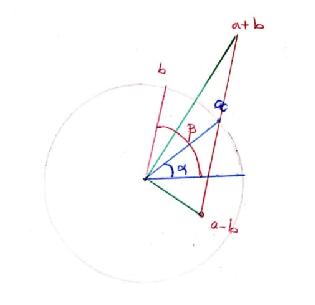
\includegraphics[width=5.29738128033583cm,height=5.12312245834973cm]{figures/Math_oraux-8.pdf}}
\end{center}

Puisque
\[ \frac{\alpha - \left( \frac{\alpha + \beta}{2} \right)}{2} = \frac{\alpha -
   \beta}{4} \not{\in} \pi \mathbb{Z} \]


On a donc $\frac{\alpha - \beta}{4} \in \Theta$.

Ainsi, par r{\'e}currence, pour tous $k, l \in \mathbb{Z}$ et pour tout $n \in
\mathbb{N}^{\ast}$
\[ \frac{k \alpha + l \beta}{2^n} \in \Theta \]


Avec $\alpha \neq 0$ ou $\beta \neq 0$, alors la suite $\left( \frac{k \alpha
+ l \beta}{2^n} \right)_{k, l \in \mathbb{Z}, n \in \mathbb{N}^{\ast}}$est
dense dans $\mathbb{R}$.

Donc, pour tout angle $\gamma$, il existe une suite de vecteurs unitaires qui
converge vers le vecteur unitaire d'angle $\gamma$.

Par fermeture, $T$ contient tous les vecteurs de tous les angles.

Ainsi, $\mathcal{C} \subset T$.

Par suite,
\[ T =\mathcal{C} \]


\tmtextbf{19.} On d{\'e}finie, $\varphi : (x, y) \longmapsto \langle A^{- 1}
x, A^{- 1} y \rangle$, avec $\langle ., . \rangle$ le produit scalaire
associ{\'e} {\`a} $\| . \|_2$.

On a bien que $\varphi$ est d{\'e}finie, et il s'agit bien d'un produit
scalaire.

Il suffit de montrer que pour tout $x \in \mathbb{R}^2$, on a $\varphi (x, x)
= \| x \|^2$ pour conclure.

Notons
\[ \Re = \{ x \in \mathcal{C} | \nobracket  \| A x \| = 1 \} \]


Il s'agit d'une partie ferm{\'e}e de $\mathcal{C}$.

D'apr{\`e}s la question 17, on a $(e_1, e_2) \in \Re$, qui est une base de
$\mathbb{R}^2$, avec $e_1 \not{=} \pm e_2$.

Pour tout $a, b \in \Re$,
\[ \| A (a + b) \|^2 + \| A (a - b) \|^2 \geqslant 4. \]


Avec $a, b \in \mathcal{C}$, alors $\| A (a + b) \|  \leqslant \| a + b \|_2$
et $\| A (a - b) \|  \leqslant \| a - b \|_2$.

Avec
\begin{eqnarray*}
  \| a + b \|^2_2 + \| a - b \|^2_2 & = & 2 (\| a \|^2_2 + \| b \|^2_2)\\
  & = & 4
\end{eqnarray*}
.

Alors,
\[ (\| a + b \|_2^2 - \| A (a + b) \|^2) + (\| a - b \|_2^2 - \| A (a - b)
   \|^2) \leqslant 0 \]


Avec $A \in \mathcal{K}$, donc $\| a + b \|^2 - \| A (a + b) \|^2 \geqslant 0$
et $\| a - b \|^2 - \| A (a - b) \|^2 \geqslant 0$.

Ainsi, $\| a - b \| _2 = \| A (a - b) \| $ et $\| a - b \| _2 = \| A (a - b)
\| $.

Par suite, \ $ \frac{a - b}{\| a - b \| _2} \in \Re$ et $ \frac{a + b}{\| a +
b \| _2} \in \Re$.

Ainsi, d'apr{\`e}s la question pr{\'e}c{\'e}dente, $\Re =\mathcal{C}$.

D'o{\`u}, pour tout $x \in \mathbb{R}^2$,
\[ \| A x \| = \| x \|_2 \]


Par suite,
\begin{eqnarray*}
  \varphi (x, x) & = & \| A^{- 1} x \|_2^2\\
  & = & \| A^{- 1} (A x) \|^2\\
  & = & \| x \|^2
\end{eqnarray*}


D'o{\`u} le r{\'e}sultat.

\

\subsubsection*{4. Alg{\`e}bres valu{\'e}es}

\tmtextbf{20.a.} Soit $x \in A$, alors par d{\'e}finition, il existe $n \in
\mathbb{N}^{\ast}$ et $a_0, \ldots, a_{n - 1} \in \mathbb{R}$ tels que
\[ x^n + a_{n - 1} x^{n - 1} + \cdots + a_1 x + a_0 = 0 \]


Par d{\'e}composition en {\'e}l{\'e}ments simples dans $\mathbb{R}$ du
polyn{\^o}me $X^n + a_{n - 1} X^{n - 1} + \cdots + a_1 X + a_0$. il existe
$b_1, \ldots, b_r, \alpha_1, \ldots, \alpha_l, \beta_1, \ldots, \beta_l \in
\mathbb{R}$ tels que
\[ X^n + a_{n - 1} X^{n - 1} + \cdots + a_1 X + a_0 = \underset{i =
   1}{\overset{r}{\prod}} (X - b_i) \underset{i = 1}{\overset{l}{\prod}} (X^2
   - \alpha_i X - \beta_i) \]


Donc,
\[ \underset{i = 1}{\overset{r}{\prod}} (x - b_i) \underset{i =
   1}{\overset{l}{\prod}} (x^2 - \alpha_i x - \beta_i) = 0 \]


Puisque $A$ est sans diviseur de z{\'e}ro, il existe $i \in \llbracket 1, r
\rrbracket$ tel que $x = b_i$ ou bien il existe $i \in \llbracket 1, l
\rrbracket$ tel que $x^2 = \alpha_i x + \beta_i$.

Dans le premier cas, on a $x^2 = b_i x \in x +\mathbb{R}x$.

Dans le deuxi{\`e}me cas, on a $x^2 \in x +\mathbb{R}x$.

Ainsi, dans tous les cas, $x^2 \in x +\mathbb{R}x$.

D'o{\`u} le r{\'e}sultat.

\

\tmtextbf{20.b.} Puisque $A \neq \mathbb{R}$, il existe $a, b \in \mathbb{R}$
tels que $x^2 = a x + b$ avec $a^2 + 4 b < 0$.

Ainsi,
\begin{eqnarray*}
  \left( x - \frac{a}{2} \right)^2 & = & b + \frac{a^2}{4}\\
  & = & \frac{a^2 + 4 b}{4}
\end{eqnarray*}


On pose
\[ y = \frac{2}{\sqrt{- a^2 - 4 b}} \left( x - \frac{a}{2} \right) \]


On a
\[ \mathbb{R}+\mathbb{R}x =\mathbb{R}+\mathbb{R}y \]


car $(y, 1)$ est $\mathbb{R}$-libre.

D{\'e}finissons $\varphi : a + y b \in \mathbb{R}+\mathbb{R}x \longmapsto a +
i b.$ On a $\varphi$ est bien d{\'e}finie et bijective (par la lib{\'e}rt{\'e}
de $(1, y)$), et de plus, pour tous $a + b y, c + d y \in
\mathbb{R}+\mathbb{R}x$, on a :
\begin{eqnarray*}
  \varphi ((a + b y) + (c + d y)) & = & (a + c) + i (b + d) y\\
  & = & \varphi (c + d y) + \varphi \nobracket (c + d y \nobracket)
\end{eqnarray*}


et
\begin{eqnarray*}
  \varphi ((a + b y) (c + d y)) & = & \varphi (a c + (b c + a d) y - b d )\\
  & = & a c - b d + i (b c + a d)\\
  & = & \varphi (a + b y) \varphi (c + d y)
\end{eqnarray*}


Donc $\varphi$ est un morphisme d'alg{\`e}bre bijectif.

\

\tmtextbf{21.} Montrons qu'il existe $i_A \in A$ tel que $i^2_A = - 1$.

Pour tout $x \in A$, on a $x^2 \in \mathbb{R}+\mathbb{R}x$, donc il existe
$a_x, b_x \in \mathbb{R}$ tels que $x^2 = a_x x + b_x$.

Supposons que pour tout $x \in A$, $a_x^2 + 4 b_x \geqslant 0$.

Alors
\[ \left( x - \frac{a_x - \sqrt{a_x^2 + 4 b_x}}{2} \right) \left( x -
   \frac{a_x + \sqrt{a_x^2 + 4 b_x}}{2} \right) = 0 \]


Or, $A$ est sans diviseur de z{\'e}ro, donc soit $x = \frac{a_x - \sqrt{a_x^2
+ 4 b_x}}{2} \in \mathbb{R}$, soit $x = \frac{a_x + \sqrt{a_x^2 + 4 b_x}}{2}
\in \mathbb{R}$.

Cela implique que $A =\mathbb{R}$, ce qui est absurde.

Ainsi, il existe $x \in \mathbb{R}$ et $a, b \in \mathbb{R}$ tels que $x^2 - a
x - b = 0,$avec $a^2 + 4 b < 0$.

On a alors
\begin{eqnarray*}
  \left( x - \frac{a}{2} \right)^2 & = & b + \frac{a^2}{4}\\
  & = & \frac{a^2 + 4 b}{4}
\end{eqnarray*}


On pose
\[ i_A = \frac{2}{\sqrt{- a^2 - 4 b}} \left( x - \frac{a}{2} \right) \]

On a alors $i^2_A = - 1$.

\

\tmtextbf{22.a.} Soient $x, y \in A$, on a :
\begin{eqnarray*}
  T (x y) & = & i_A x y i_A\\
  & = & - i_A x (i_A i_A) y i_A\\
  & = & - (i_A x i_A) (i_A y i_A)\\
  & = & - T (x) T (y)
\end{eqnarray*}


\tmtextbf{22.b.} On a, pour tout $x \in A$,
\begin{eqnarray*}
  T \circ T (x) & = & i_A (i_A x i_A) i_A\\
  & = & x\\
  & = & \tmop{id} (x)
\end{eqnarray*}


Donc $T \circ T$=id, et ainsi
\[ X^2 - 1 = (X - 1) (X + 1) \]


est un polyn{\^o}me annulateur de $T$. De plus, $X + 1$ et $X - 1$ sont
premiers entre eux. D'apr{\`e}s le th{\'e}or{\`e}me de d{\'e}composition des
noyaux, on a :
\[ A = \ker (T - \tmop{id}) \oplus \ker (T + \tmop{id}) \]

\tmtextbf{23.} Montrons que $\ker (T + \tmop{id}) = U$

Soit $x \in \tmop{Ker} (T + \tmop{id}) \backslash \{ 0 \} \nobracket$. Alors
$T (x) = - x$, donc $x = - i_A x i_A$, ainsi $i_A x = x i_A$.

Donc $x$ et $i_A$ commutent. Par suite,
\[ (i_A x )^2 = - x^2 \]


En particulier, $i_A x \not{\in} \mathbb{R}$, ce qui implique que $(i_A x, 1)$
est une base de $\mathbb{R}+\mathbb{R}x$.

Ainsi, il existe $a, b \in \mathbb{R}$ tels que
\[ x = a + b i_A \in U \]


R{\'e}ciproquement, si $x \in U$, alors il existe $(a, b) \in \mathbb{R}^2$
tel que
\[ x = a + b i_A \]


Donc
\begin{eqnarray*}
  T (x) & = & i_A (a + b  i_A) i_A\\
  & = & i_A a i_A - i_A b\\
  & = & a i_A i_A - b i_A\\
  & = & - a - b i_A\\
  & = & - x
\end{eqnarray*}
Donc
\[ x \in \tmop{Ker} (T + \tmop{id}) \]
Ainsi, $\ker (T + \tmop{id}) = U$, et puisque A n'est pas isomorphe {\`a}
$\mathbb{C}$ et que Ker(T+id) est de dimension 2, alors Ker(T-id) n'est pas
r{\'e}duit {\`a} z{\'e}ro.

\

\tmtextbf{24.} Fixons $\beta \in \tmop{Ker} (T - \tmop{id}) \backslash
\nobracket \{ 0 \}$.

\tmtextbf{24.a.} Montrons que l'application $x \longmapsto \beta x$ envoie
$\ker (T - \tmop{id})$ dans $\ker (T + \tmop{id})$.

Soit $x \in \tmop{Ker} (T - \tmop{id})$, donc $T (x) = x$.

Or, $\beta \in \tmop{Ker} (T - \tmop{id})$, donc $T (\beta) = \beta$.

D'apr{\`e}s la question 22.a, on a :
\begin{eqnarray*}
  T (\beta x) & = & - T (\beta) T (x)\\
  & = & - \beta x
\end{eqnarray*}


Par suite, $\beta x \in \ker (T + \tmop{id})$, donc $x \longmapsto \beta x$
envoie $\ker (T - \tmop{id})$ dans $\ker (T + \tmop{id})$.

D'apr{\`e}s la question pr{\'e}c{\'e}dente, on a $\beta \ker (T - \tmop{id})
\subset U$.

Ainsi, $\dim_{\mathbb{R}} \ker (T - \tmop{id}) \leqslant \dim_{\mathbb{R}} U$

De m{\^e}me $x \longmapsto \beta x$ envoie $\ker (T + \tmop{id})$ dans $\ker
(T - \tmop{id})$, donc $\dim_{\mathbb{R}} (\ker (T - \tmop{id})) \geqslant
\dim_{\mathbb{R}} U$.

On en d{\'e}duit que
\[ \dim_{\mathbb{R}} U = \dim_{\mathbb{R}} \ker (T - \tmop{id}) \]


Par suite, $U = \ker (T - \tmop{id})$.

\

\tmtextbf{24.b.} Montrons que $\beta^2 \in] - \infty, 0 [$.

D'apr{\`e}s ce qui pr{\'e}c{\'e}de, on a $\beta \ker (T - \tmop{id}) \subset
U.$

Donc, $\beta^2 \ker (T - \tmop{id}) \subset \beta U = \ker (T - \tmop{id})$.

Comme $\ker (T - \tmop{id}) \not{=} \{ 0 \}$, il en r{\'e}sulte que $\beta^2
\in \mathbb{R}$.

Supposons par l'absurde que $\beta^2 > 0$. Alors, $\beta = \sqrt{\beta^2} \in
\mathbb{R}$, donc $\beta U = U$.

Ainsi,
\begin{eqnarray*}
  A & = & U + \beta U\\
  & = & U
\end{eqnarray*}


Or, $U$ est isomorphe {\`a} $\mathbb{C}$, ce qui est absurde, car $A$ n'est
pas isomorphe {\`a} $\mathbb{R}$ ni {\`a} $\mathbb{C}$.

D'o{\`u} le r{\'e}sultat.

\

\tmtextbf{24.c.} On a $i_A \in \tmop{Ker} (T + \tmop{id})$, donc $\beta i_A
\in \beta U$. Ainsi, $(\beta, \beta  i_A)$ est une base de $\beta U$, et $(1,
i_A)$ est une base de $U$. Par somme directe, on a $(1, i_A, \beta, \beta
i_A)$ est une base de $A$.

Donc $A$ est isomorphe {\`a} $\mathbb{H}$. (car $\dim_{\mathbb{R}} \mathbb{H}=
4$)

\

\tmtextbf{25.} Soient $x, y \in A$ tels que $x y = y x$ et tels que $V
=\mathbb{R}x +\mathbb{R}y$ soit de dimension 2 sur $\mathbb{R}$.

Montrons que pour tout $u, v \in V$, on a
\[ \| u + v \|^2 + \| u - v \|^2 \geqslant 4 \| u \| . \| v \| \]


Soient $u, v \in \mathbb{R}x +\mathbb{R}y$. Puisque $x, y$ commutent, alors
$u, v$ commutent {\'e}galement, en tant que polyn{\^o}mes $x$et $y$. Or,
\[ \| u + v \|^2 = \| (u + v)^2 \| \infixand \| u - v \|^2 = \| (u - v)^2 \|
\]


Par l'in{\'e}galit{\'e} triangulaire inverse, on a
\begin{eqnarray*}
  \| u + v \|^2 + \| u - v \|^2 & \geqslant & \| (u + v)^2 - (u - v)^2 \|\\
  & \geqslant & 4 \| u \| . \| v \|
\end{eqnarray*}


Montrons que la restriction de $\| . \|$ {\`a} $V$ provient d'un produit
scalaire sur $V$.

On a $V = x\mathbb{R}+ y\mathbb{R}$ de dimension $2$, donc $V$ est isomorphe
{\`a} $\mathbb{R}^2$.

Il existe un isomorphisme d'espaces vectoriels $\varphi : \mathbb{R}^2
\rightarrow V$.

On a, pour tout $x, y \in \mathbb{R}^2$,
\[ \| \varphi (x) + \varphi (y) \|^2 + \| \varphi (x) - \varphi (y) \|^2
   \geqslant 4 \| \varphi (x) \| . \| \varphi (y) \| \]


Ainsi,
\[ \| \varphi (x + y) \|^2 + \| \varphi (x - y) \|^2 \geqslant 4 \| \varphi
   (x) \| . \| \varphi (y) \| \]


Avec $\psi : x \in \mathbb{R}^2 \longmapsto \| \varphi (x) \|$ est une norme
sur $\mathbb{R}^2$, en effet, pour tout $x, y \in \mathbb{R}^2$ et $\lambda
\in \mathbb{R}$, on a

Si $\| \varphi (x) \| = 0$, alors $\varphi (x) = 0$, et par injectivit{\'e},
on a $x = 0$.

De plus, $\| \varphi (\lambda x) \| = | \lambda | \| \varphi (x) \|$ et $\|
\varphi (x + y) \| = \| \varphi (x) + \varphi (y) \| \leqslant \| \varphi (x)
\| + \| \varphi (y) \|$.

D'apr{\`e}s le th{\'e}or{\`e}me $A$, on a $x \longmapsto \| \varphi (x) \|$
provient d'un produit scalaire $\langle . | \nobracket . \rangle$.

Notons
\[ \zeta : (u, v) \in V \longmapsto \langle \varphi^{- 1} (u), \varphi^{- 1}
   (v) \rangle \]
.

On a $\zeta$ est sym{\'e}trique. De plus, pour tout $u \in V$,
\begin{eqnarray*}
  \zeta (u, u) & = & \| \varphi (\varphi^{- 1} (u)) \|\\
  & = & \| u \|\\
  & \geqslant & 0
\end{eqnarray*}


Donc $\zeta$ est positif.

Par lin{\'e}arit{\'e} de $\varphi^{- 1}$, on a $\zeta$ est bilin{\'e}aire.

Et par injectivit{\'e}, $\zeta$ est d{\'e}finie.

Donc $\zeta$ d{\'e}finie un produit scalaire sur $V$.

$\| . \|$ provient de $\zeta$.

D'o{\`u} le r{\'e}sultat.

\

\tmtextbf{26.} Soit $x \in A$. Si $x \in \mathbb{R}$, il est {\'e}vident que
\[ x^2 \in \mathbb{R}+\mathbb{R}x \]


Supposons que $x \in A \backslash \mathbb{R} \nobracket$, alors $V = x
+\mathbb{R}x$ est de dimension 2.

D'apr{\`e}s la question pr{\'e}c{\'e}dente, $\| . \|$ provient d'un produit
scalaire sur $V$.

Notons $y$ un vecteur orthogonal non nul {\`a} $1$ dans $V$.

Ainsi, on a $(1, y)$ forme une base de $V$.

Donc il existe $a, b \in \mathbb{R}$ tels que $x = a + b y$.

Ainsi,
\[ x^2 = a^2 + 2 a b y + y^2 \]


Avec :
\begin{eqnarray*}
  \langle 1, y^2 \rangle & = & \frac{1}{2} (\| y^2 \|^2 + 1 - \| y^2 - 1
  \|^2)\\
  & = & \frac{1}{2} (\| y^2 \|^2 + 1 - \| y  - 1 \|^2 \| y  + 1 \|^2)\\
  & = & \frac{1}{2} (\| y  \|^4 + 1 - (\| y  \|^2 + 1)^2)\\
  & = & \left. \frac{1}{2} (\| y  \|^4 + 1 - \| y  \|^4 - 2 \| y \|^2 - 1
  \nobracket \right)\\
  & = & - \| y^2 \|\\
  & = & - \| 1 \|^2 \| y^2 \|
\end{eqnarray*}


Et donc, d'apr{\`e}s le cas d'{\'e}galit{\'e} dans l'in{\'e}galit{\'e} de
Cauchy-Schwarz, on a $y^2 \in \mathbb{R}$.

D'o{\`u} :
\begin{eqnarray*}
  x^2 & \in & \mathbb{R}+\mathbb{R}_y\\
  & = & \mathbb{R}+\mathbb{R}_x
\end{eqnarray*}


27. D'apr{\`e}s la question pr{\'e}c{\'e}dente, on a A est alg{\'e}brique (car
Pour tout $x \in \mathbb{R}$, il existe $a, b \in \mathbb{R}$ tels que $x^2 = ax + b$).

De plus, A est sans diviseur de z{\'e}ro : en effet, pour $x, y \in A$ tels
que $x y = 0,$ on alors

$\|x\|\|y\|=\|x y\|= 0$

\ \ \ \ \

Par cons{\'e}quent $\|x\|= 0$ ou $\|y\|= 0.$

Par suite $x = 0$ou $y = 0$.

Ainsi, d'apr{\`e}s le th{\'e}or{\`e}me $B$, $A$ est isomorphe {\`a}
\ensuremath{\mathbb{R}}, \ensuremath{\mathbb{C}} ou \ensuremath{\mathbb{H}}.

D'o{\`u} le th{\'e}or{\`e}me $C$.